\chapter{The LUX-ZEPLIN Dark Matter Experiment}\label{chap:LZExperiment}
The LZ experiment is currently the leading dark matter direct detection experiment in the search for WIMPs. The detector is located on the 4,850~ft level (4,300~mwe) of the Sanford Underground Research Facility (SURF) in the Homestake Mine (Lead, SD) \cite{LZNIMA}. At the core of the experiment is a dual-phase Time Projection Chamber (TPC) which is sensitive to low -energy nuclear recoils (NR), the signal which is produced through WIMPs interacting with liquid noble gases. One of the main backgrounds in a WIMP search are neutrons as they also interact through nuclear recoils and thus LZ employs an active veto system to remove them. Theoretically WIMPs will only interact with the xenon target however neutrons would interact in both the TPC and veto detectors. The TPC is housed within a vacuum insulated cyrostat with a layer of liquid xenon (Skin) which acts as high voltage stand-off, this region is also instrumented with PMTs and is part of the active veto system. The LXe skin is used to veto mostly gamma ray interactions within the TPC volume, also being sensitive to neutrons. The cryostat is surrounded near hermetically by ten acrylic vessels filled with Gadolinium-loaded liquid scintillator (GdLS). The GdLS is observed by 120 PMTs and stands within 238t of DI water which provides shielding to the detector. A schematic of the detector is shown in \autoref{fig:LZDetector}.
\begin{figure}
    \centering
    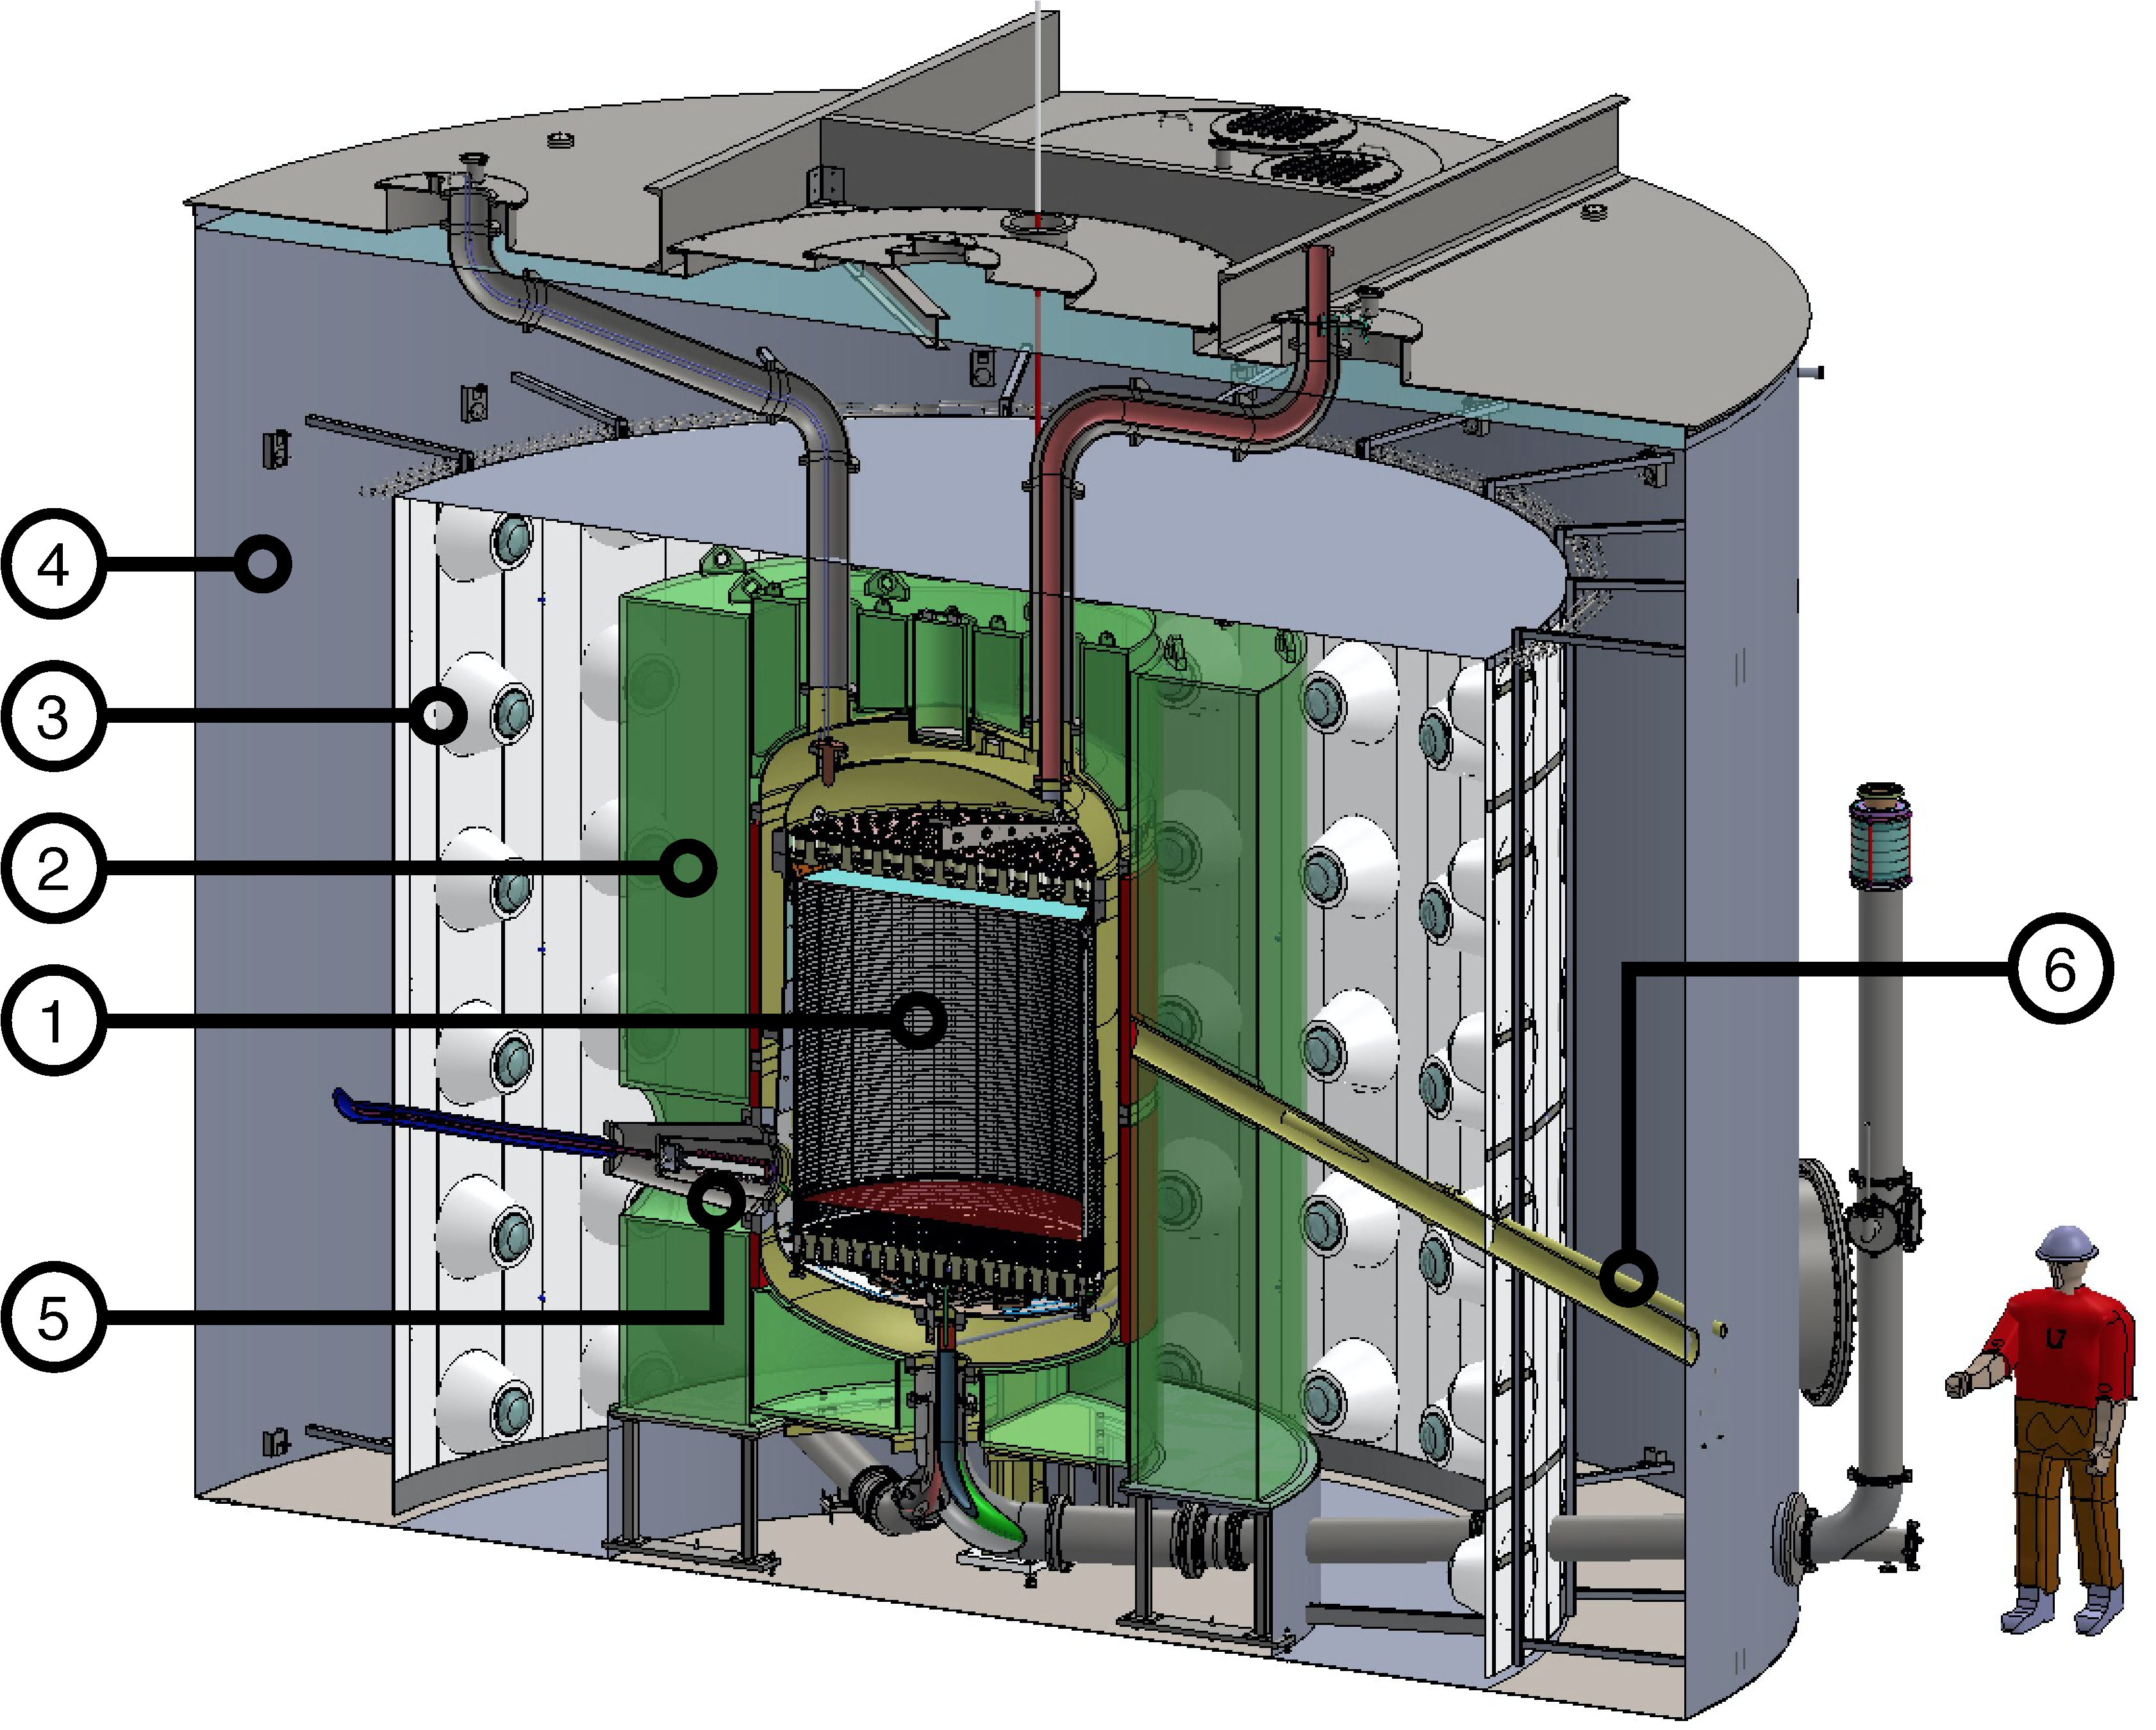
\includegraphics[width=0.7\linewidth]{figures/LZ/LZSchematic.pdf}
    \caption{Schematic of the LZ detector showcasing the major subsystems. At the center is the liquid xenon TPC (1), monitored by two arrays of PMTs and serviced by various cable and fluid conduits (upper and lower). The TPC is contained in a double-walled vacuum insulated titanium cryostat and surrounded on all sides by a GdLS Outer Detector (2). The cathode high voltage connection is made horizontally at the lower left (5). The GdLS is observed by a suite of 8” PMTs (3) standing in the water (4) which provides shielding for the detector. The pitched conduit on the right (6) allows for neutron calibration sources to illuminate the detector \cite{LZNIMA}.}
    \label{fig:LZDetector}
\end{figure}
\section{Liquid Xenon Time Projection Chamber}\label{sec:LXeTPC}
The LZ TPC holds 7~t (5.6~t fiducial) of liquid xenon (LXe) above its cathode, there is an additional thin layer (8~mm thick) of gaseous xenon (GXe) at the top of the liquid. The volume measures approximately 1.5~m in height and diameter and the walls of the TPC are made from PTFE to improve light collection efficiency \cite{LZNIMA}. The TPC, Skin and Xe payload are housed within the Inner Cryostat Vessel (ICV) and the Outer Cryostat Vessel (OCV) provides a vacuum jacket for insulation. Both cryostat vessels are made from low radioactivity titanium \cite{LZ:2017iwn}. When a particle scatters off a LXe atom a prompt scintillation signal (S1) is produced alongside free elections, via ionisation of the LXe atom. Through the application of an electric field, the free electrons drift to the LXe surface and are extracted in the GXe layer. As the electrons accelerate through the GXe layer, a proportional amount of scintillation light (S2) is produced. Light produced from these particle interactions is observed by a top and bottom array of 3-inch Hamamatsu R11410–22 PMTs, 494 in total. Using both the S1 and S2 signals, position reconstruction techniques can be used to determine the $xyz$-position of the particle interaction. The time difference between the S1 and S2 signals combined with the drift velocity is used to determine the $z$-position of the interaction whilst the hit pattern of the S2 signal in the top PMT array provides $xy$-position. The operating principle of a TPC can be seen in \autoref{fig:TPCCartoon}.
\begin{figure}
     \centering
     \begin{subfigure}{0.47\textwidth}
         \centering
         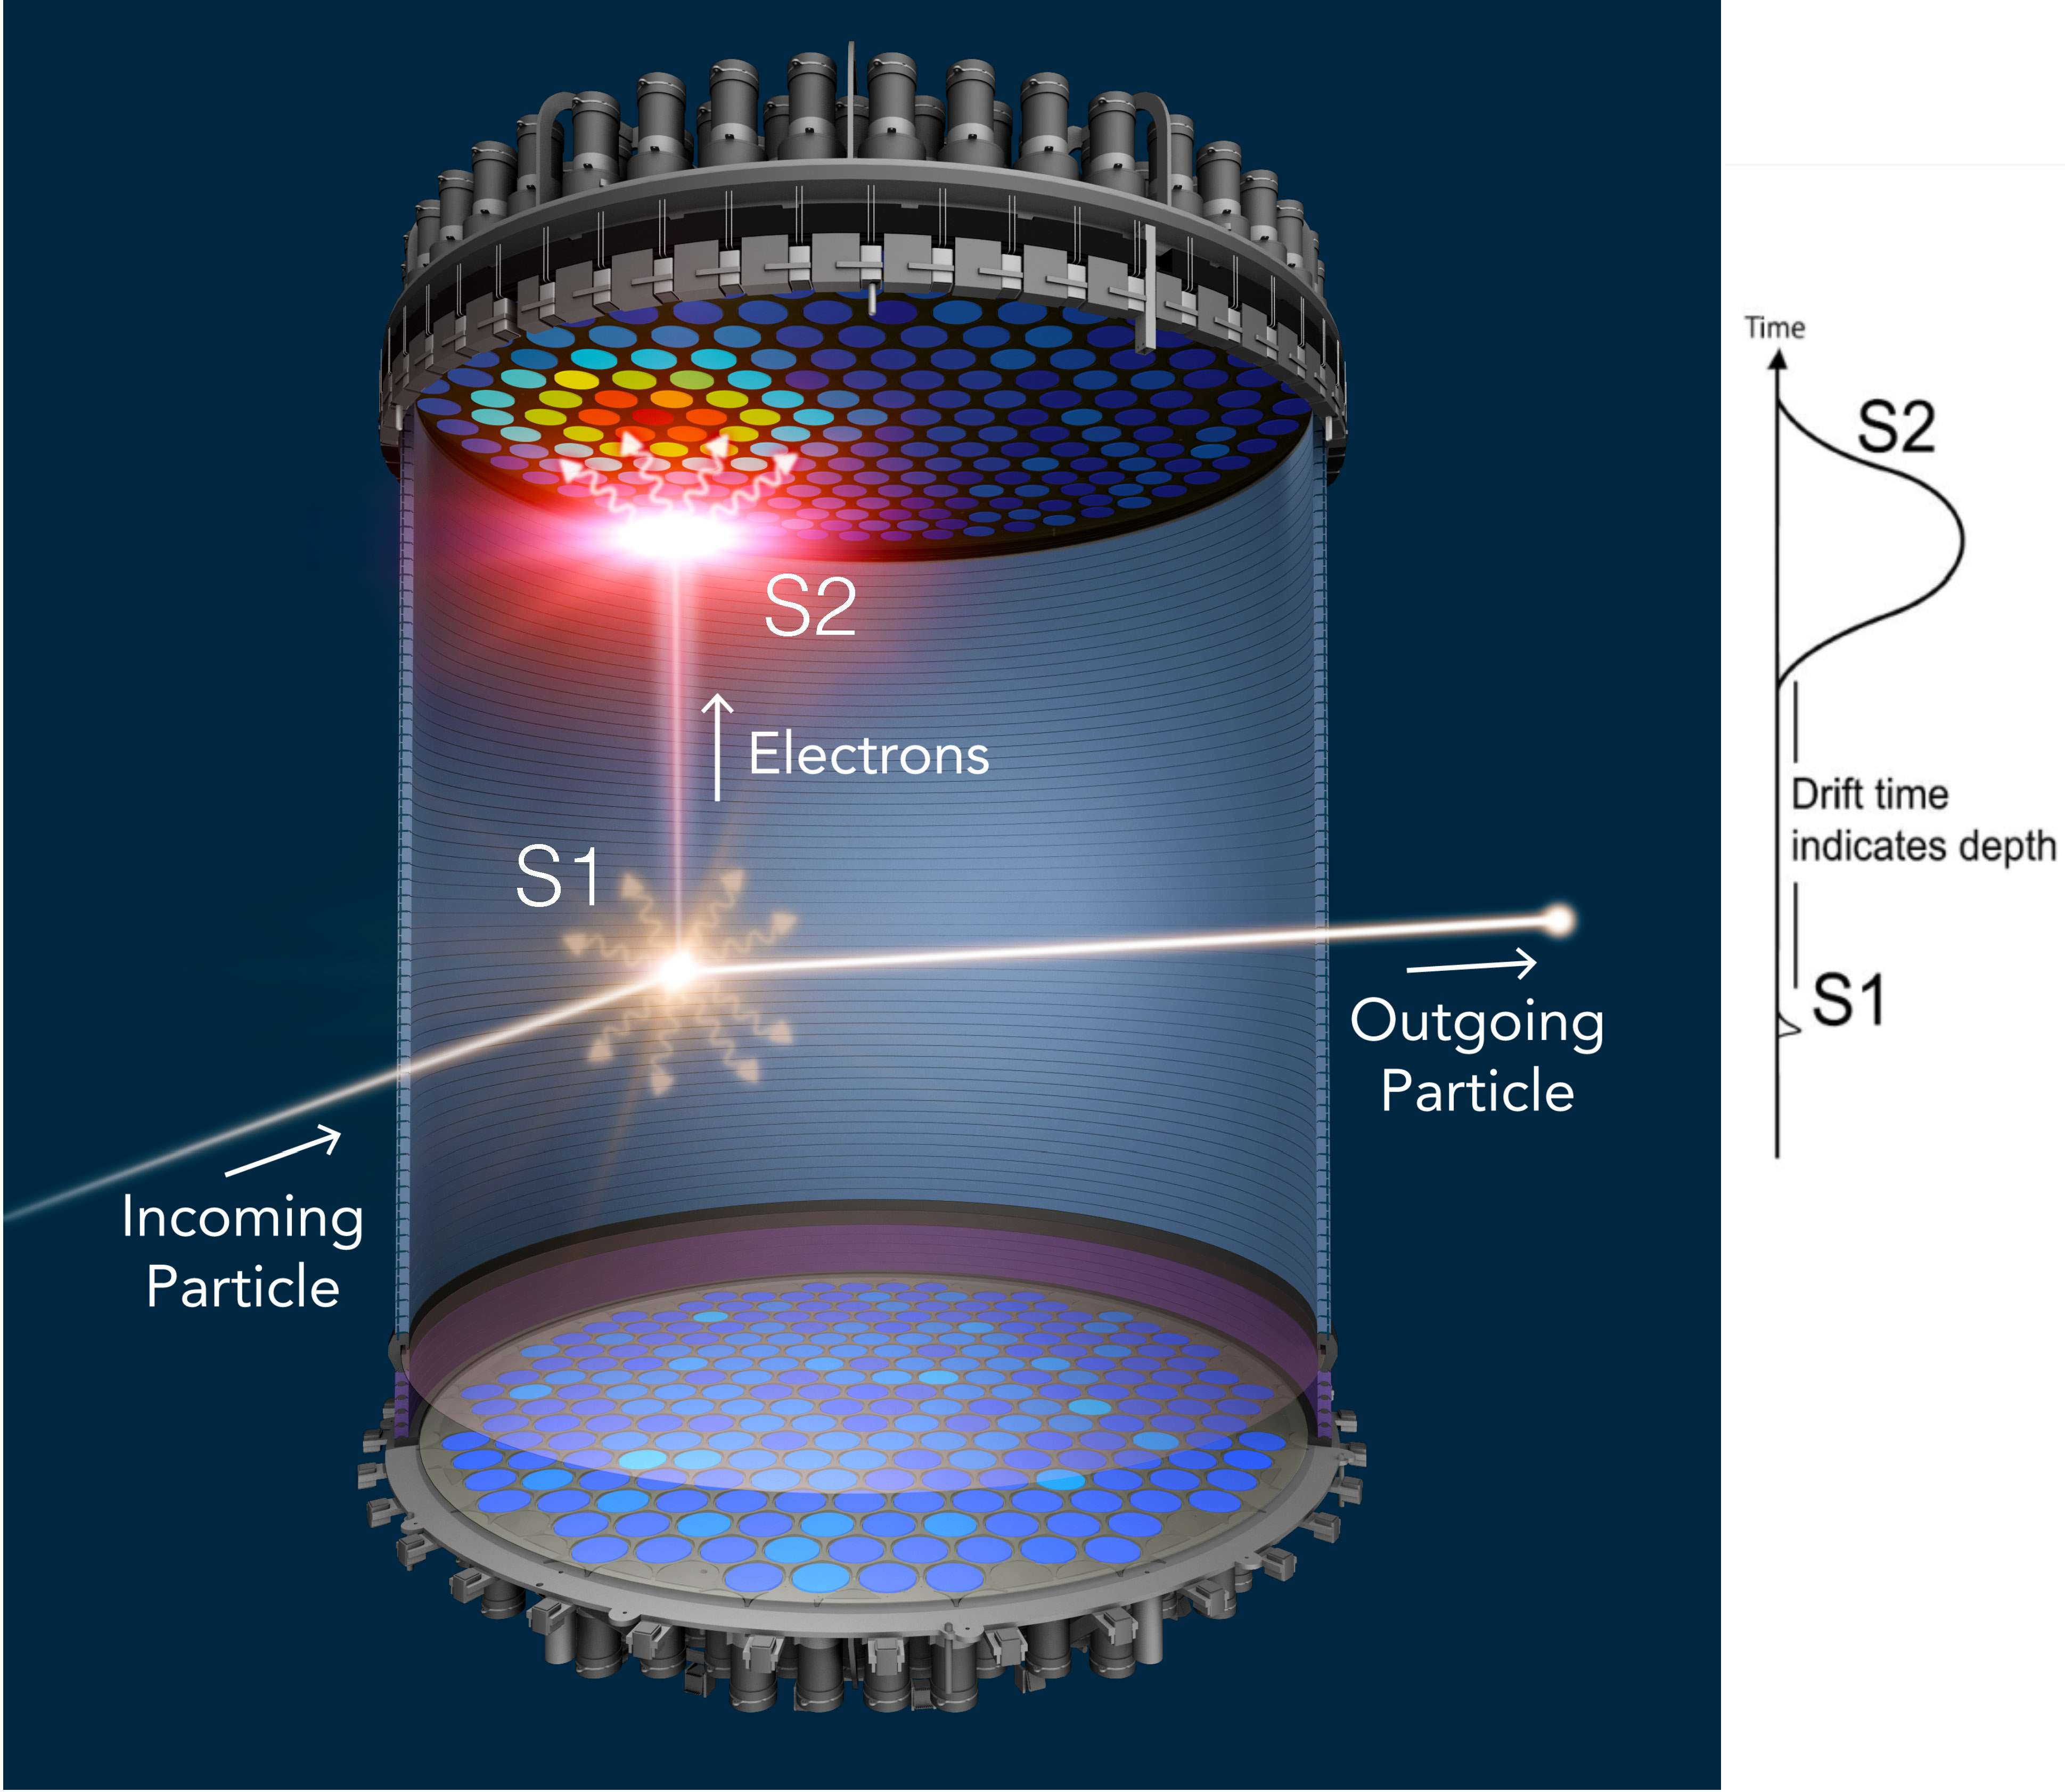
\includegraphics[width=\textwidth]{figures/LZ/IDOf_Xe_TPC2.jpg}
         \caption{}
         \label{fig:TPCCartoon}
     \end{subfigure}
     %\hfill
     \begin{subfigure}{0.47\textwidth}
         \centering
         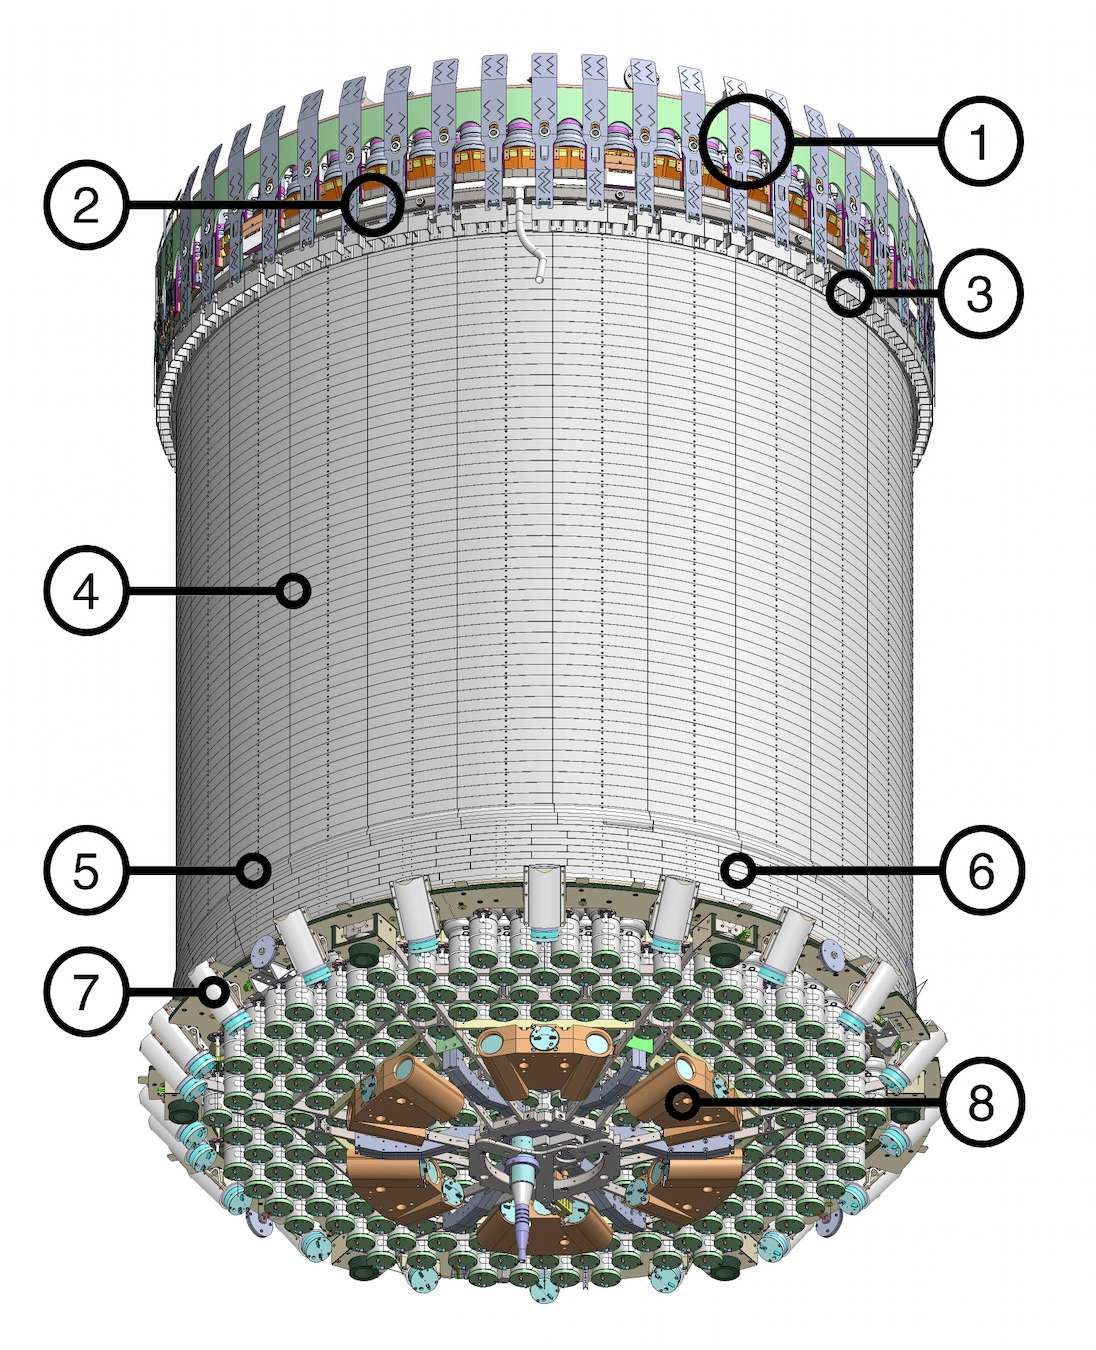
\includegraphics[width=0.5\textwidth]{figures/LZ/CAD_TPC.jpg}
         \caption{}
         \label{fig:CAD_TPC}
     \end{subfigure}
     \caption{Dual phase liquid noble TPC operating principle and components. \textbf{\ref{fig:TPCCartoon}:} Each particle interaction with the LXe atoms produces two signals: an initial prompt scintillation (S1) and a second, delayed one from ionisation (S2) \cite{LZTDR}. The combination of these two signals allows for precise 3D position reconstruction and discrimination between nuclear and electron recoils.
     \textbf{\ref{fig:CAD_TPC}:} CAD drawing of the TPC \& Skin components: 1-Top PMT array; 2-Gate-anode and weir region (liquid level); 3-Side skin PMTs (1-inch); 4-Field cage; 5-Cathode ring; 6-Reverse field region; 7-Lower side skin PMTs (2-inch); 8-Dome skin PMTs (2-inch) \cite{LZNIMA}.}
\end{figure}

\subsection{Particle-Xenon interactions within a TPC}
As a particle traverses the LXe volume it can interact with either the atomic nucleus, producing a nuclear recoil (NR), or with the surrounding electron cloud, producing an electronic recoil (ER). Both processes result in the pair of signals discussed in \autoref{sec:LXeTPC}. The S1 signal is produced via the following mechanism. The excited Xe atom, $Xe^{*}$, combines with a nearby ground state $Xe$ atom to form an excimer state, $Xe
_{2}^{*\nu}$, which is both an electronically and vibrationally excited molecule. Through collisions with other Xe atoms, energy in the vibrational modes of the excimer is lost. The excited pair de-excites further as the electronic excitation energy is released as a pair of vacuum-ultraviolet (VUV), at a mean wavelength of 178~nm \cite{Schumann:2014uva}.
The $Xe$ atom also undergoes ionisation due to the displacement of the nucleus during the collision releasing electrons. A positively charged $Xe^{+}$ ion combines with a neutral Xe atom to form a positively charged dimer $Xe^{+}_{2}$. Most of the electrons that are emitted in the ionisation are drifted away from the collision site by the applied electric field. However some of the ionised electrons produced in the cascade recombine with the molecule prior to it splitting to form a highly excited $Xe$ atom. A final series of relaxation occurs in a similar manner to the excitation luminescence excimer. A schematic which describes the process of producing the S1 and S2 signal can be seen in \autoref{fig:XenonSigalProduction}.
\begin{figure}
    \centering
    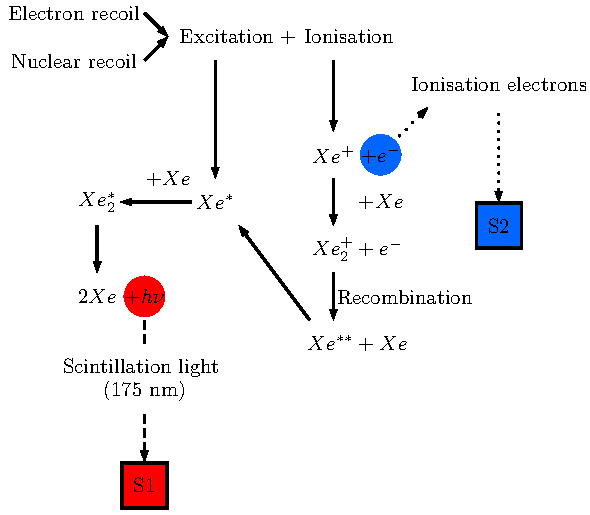
\includegraphics[width=0.6\linewidth]{figures/LZ/Xenon_interaction.pdf}
    \caption{A schematic of the signal production and collection in a dual phase xenon time}
    \label{fig:XenonSigalProduction}
\end{figure}

To understand what particle has passed through the LXe it is important to determine the energy deposited in interaction with the Xe atom. This can be described using the following equation:
\begin{equation}
    E=\frac{W}{L}(n_{ex}+n_{i})
    \label{eqn:EnergyRec_noG}
\end{equation}
Where W is the average energy required to produced either one scintillation photon or ionisation electron, which has been measured to be $13.7\pm0.4~eV$ \cite{Goetzke:2016lfg, Dahl:2009nta}.
L is referred to as the "Lindhard factor" or "quenching" accounting for the reduction of produced light and charge as energy is lost at heat. For electron recoils L is taken as unity, this implies that the heat-loss is constant with energy allowing it to be absorbed into the value of W \cite{Rischbieter:2022}. The Lindhard factor for nuclear recoils is observed to be a function of deposited energy as the interaction energy is not linearly related to the observed total quanta \cite{Sorensen:2011bd}.
$n_{ex}$ and $n_{i}$ represent the number of excited atoms and ionised atoms and are proportional to pulse area of the S1 and S2 pulses observed in the TPC respectively. The constants of proportionality are $g_1$ and $g_2$ and represent the S1 light collection efficiency and the electron extraction efficiency of the detector respectively. Thus \autoref{eqn:EnergyRec_G} can be modified to describe the energy deposition using:
\begin{equation}
    E=\frac{W}{L}(\frac{S1}{g_1}+\frac{S2}{g_2})
    \label{eqn:EnergyRec_G}
\end{equation}

\subsection{NR and ER Discrimination}
The ratio of energy distribution between light and charge differs between NRs and ERs. This can be directly observed through the S1 and S2 pulse areas produced from the interactions, particularly the ratio, $log_{10}(S2)/S1$. This method demonstrates $95~\%$ discrimination against ER with a $50~\%$ \cite{lzSens}. This is key for the search for WIMPs where we would expect to observe an NR when a WIMP passes through the TPC. However, the dominant backgrounds such as $\beta$-decays from Rn daughter isotopes and \textsuperscript{85}Kr and $\gamma$ radiation from detector components all produce ER events in the LXe. Both ER and NR events form distinctive band structure $log_{10}(S2)/S1$ space, as shown in \autoref{fig:NRERBandExample}, where the width of the bands is due to electron-ion recombination at the interaction site whilst the overall separation is due to the ratio of ionisation to excitation in the interaction \cite{Dahl:2009nta}.

\begin{figure}
    \centering
    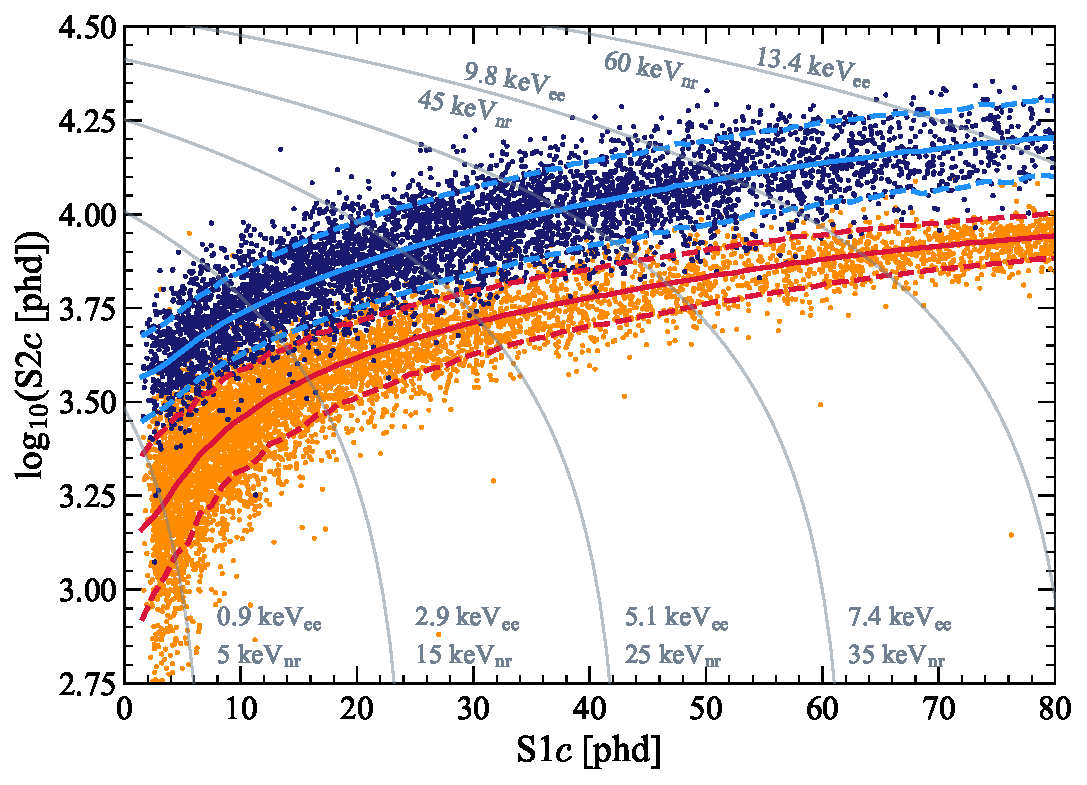
\includegraphics[width=0.75\linewidth]{figures/LZ/SR1WS_calOnly_0629.pdf}
    \caption{Discrimination between ER and NR can be seen in LZ calibration events in $log_{10}S2_{c}-S1_{c}$ for the tritium source (dark blue points, 5343 events) and the DD neutron source (orange points, 6324 events). Solid blue (red) lines indicate the median of the ER (NR) simulated distributions, and the dotted lines indicate the 10~\% and 90~\% quantiles. Thin gray lines show contours of constant electron-equivalent energy ($keV_{ee}$) and nuclear recoil energy ($keV_{nr}$) \cite{LZ:2022lsv}.}
    \label{fig:NRERBandExample}
\end{figure}

\section{Xenon Skin}
The TPC is surrounded by a layer of LXe, the region contains around 2 tonnes of LXe between the field cage and the inner cryostat vessel \cite{LZNIMA}. The primary motivation for including this layer of LXe was to provide dielectric insulation between the two elements. Unlike Xenon-nT, LZ's main competitor, this region is instrumented for optical readout acting as a scintillation-only veto detector for gamma interactions in the TPC \cite{XENON:2024wpa}. The region is nominally known as the "Skin" and can be split into two regions: Barrel and Dome. The Barrel contains 93 1-inch Hamamatsu R5820 PMTs at the top of the Barrel looking down and 38 2-inch Hamamatsu R8778 PMTs; 20 at the bottom of the Barrel looking up, and 18 in the Dome region below the TPC \cite{LZNIMA}. The layout of the Skin PMTs with respect to the TPC can be seen in \autoref{fig:CAD_TPC}.

\section{Outer Detector}
It has been shown in previous sections that dual phase TPC has the capability to distinguish between ER and NR interactions in the LXe, however it does not have the capability to understand what particle caused the recoil. Neutrons are the primary source of NRs as they can easily scatter of the Xe nuclei and mimic a signal similar to a WIMP. Neutrons will however scatter multiple times in the TPC or nearby whereas WIMPs would not due to differences in their respective interactions cross sections. LZ has taken advantage of this principle and surrounded the TPC in a neutron detector to increases it's discrimination power on NR backgrounds. This detector is nominally known as the Outer Detector.
%and together with the Xe Skin comprises the LZ Veto System. 
The outer cryostat housing the TPC is surrounded near hermetically by ten acrylic vessels filled with  Gadolinium loaded liquid scintillator (GdLS). The GdLS is observed by 120 PMTs and stands within 238t of DI water which provides shielding to the detector. An exploded layout of these vessels can be seen in \autoref{fig:ODTanks}.
\begin{figure}
    \centering
    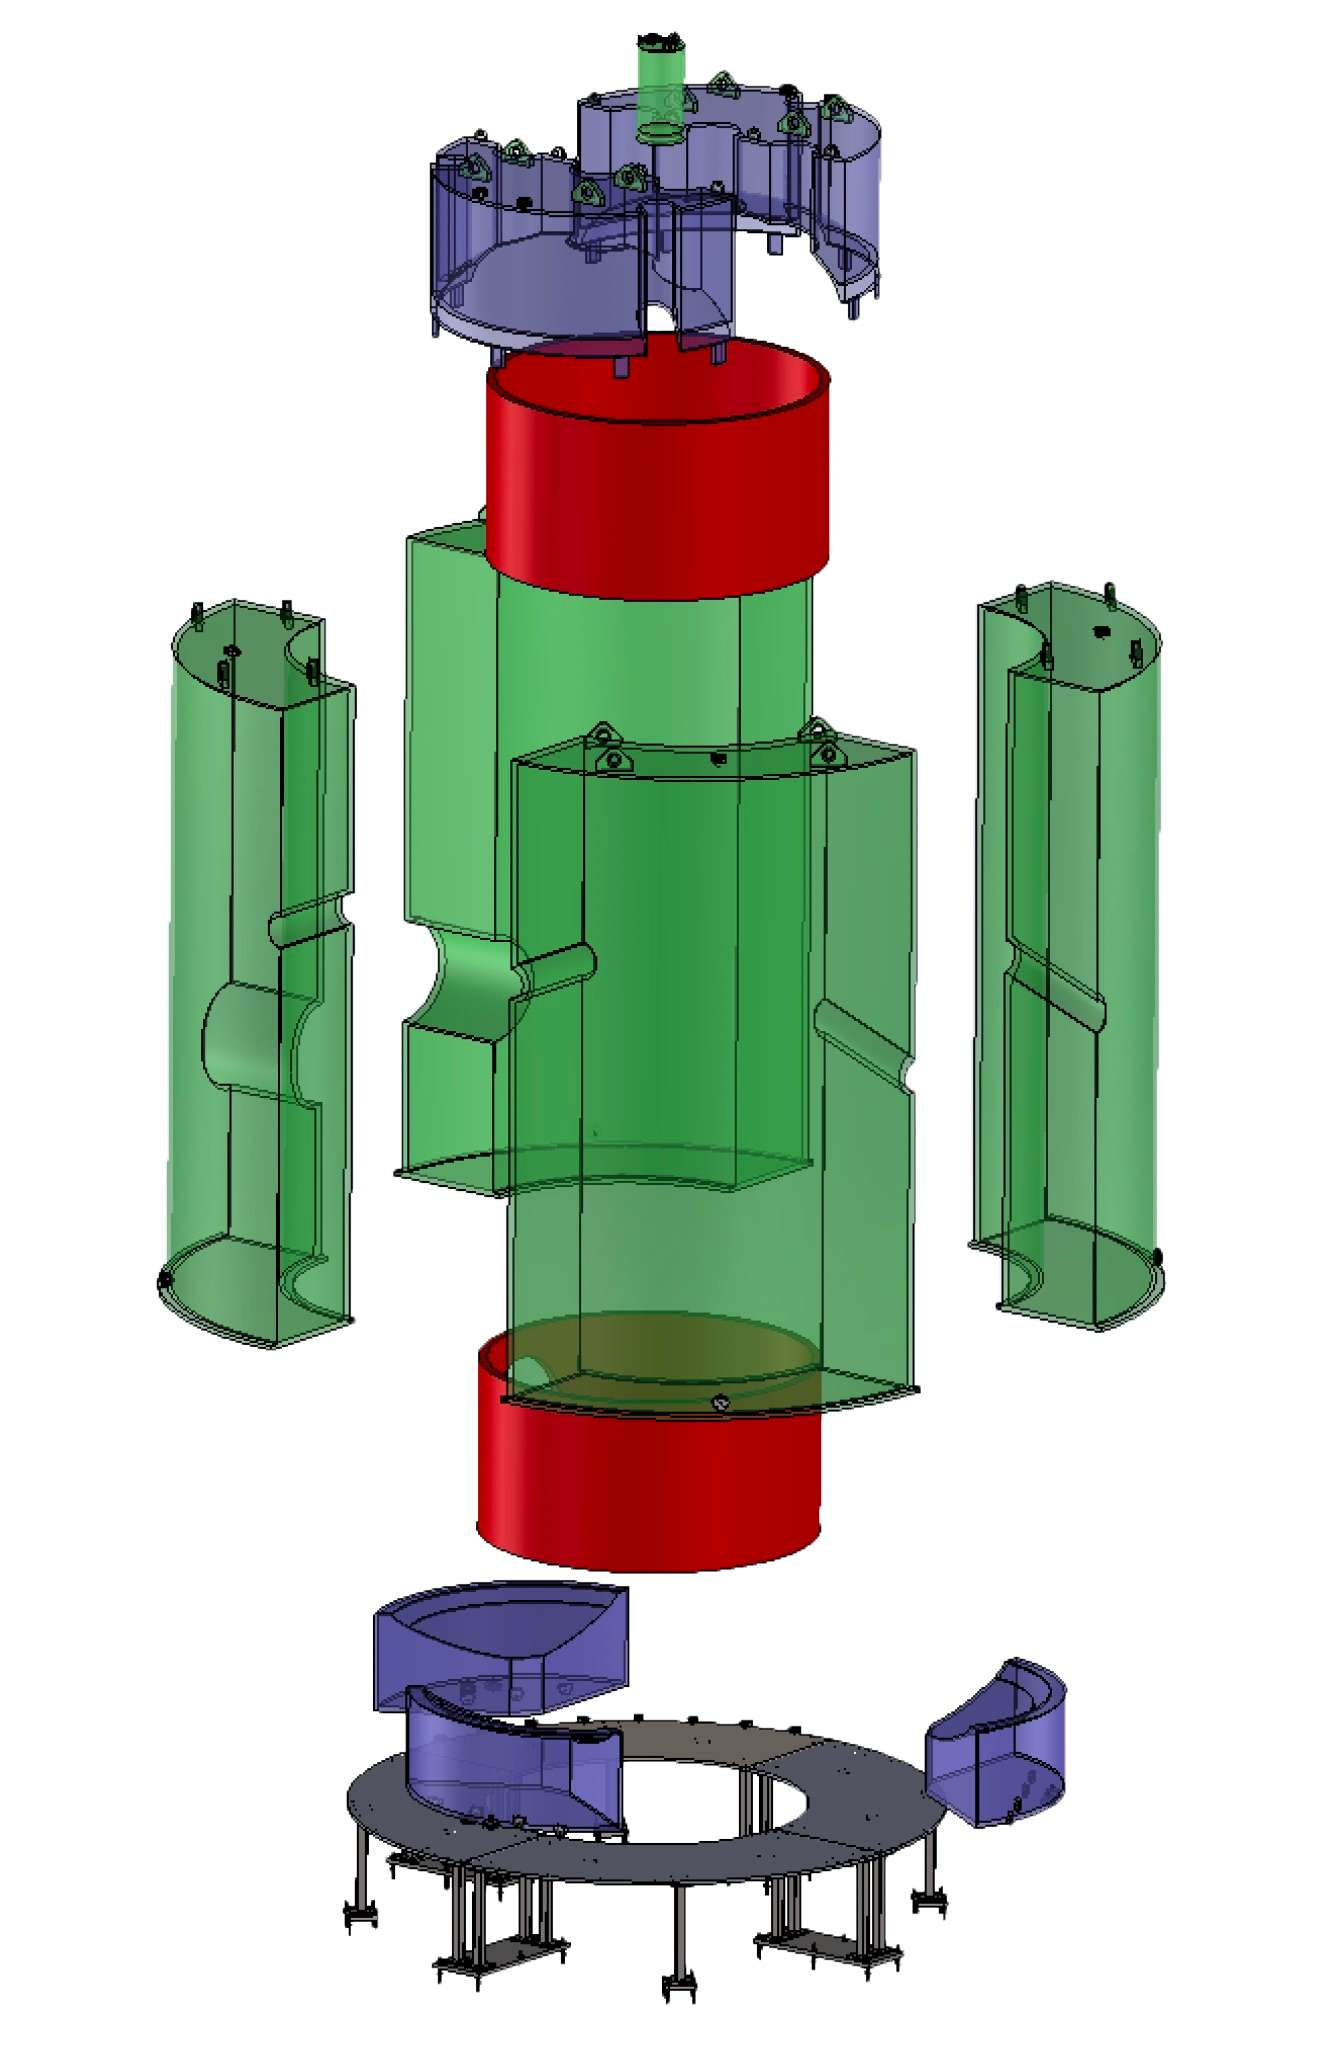
\includegraphics[width=0.5\linewidth]{figures/LZ/CAD_ODTanks.jpg}
    \caption{The Outer Detector vessels in an exploded view. The four large side vessels (SATs) are shown in green, the five small vessels (two top (TATs) and three bottom (BATs)) are shown in blue. The stainless steel base can be seen in grey and the foam water displacers in red. There is an additional small vessel shown in green at the top which is removed for photoneutron calibration source deployment \cite{LZNIMA}.}
    \label{fig:ODTanks}
\end{figure}

\subsection{Liquid Scintillator}
The primary detection medium for the OD is the GdLS, chosen for its excellent efficiency for neutrons and gammas that reach the OD \cite{LZTDR}. The composition of the GdLS mixture is shown in \autoref{tab:GdLSComp}. The base of the LS mixture is Linear-alkylbenzene (LAB), which acts as a solvent for the other components of the mixture. In addition to the LAB, the fluor 2,5-diphenyloxazole (PPO), and the wavelength shifter 1,4-bis(2-methylstyryl(benzene)) (Bis-MSB) are considered as the LS. As particles pass through the LS, the LAB component is excited as the particles deposit energy along the tracks. Through a series of chemical reactions, the excited LAB transmits energy to the fluor. As the excited fluor de-excites, it emits light with wavelengths up to 380~nm. Due to the short absorption lengths of the LS below 380~nm (approximately 1~m), Bis-MSB is included as a wavelength shifter. The Bis-MSB absorbs the photons produced by the fluor and emits photons with wavelengths between 410~nm~-~425~nm with absorption lengths over 10~m. Bis-MSB is a crucial component of the mixture as wavelengths of the emitted photons overlap with the PMT sensitivity spectrum and absorption lengths satisfy the detector geometry.
The mixture is additionally loaded with Gd with a mass fraction of $0.1~\%$. Gd has a very high $(n,\gamma)$ cross-section so improves both the efficiency and intensity of the neutron capture signal \cite{LZTDR}. Due to the effectiveness of the Gd, only a small mass fraction is needed to dominate over neutron capture on protons in the LS. To dissolve the Gd in solution with the LS it is bound to a chelating agent, 3,5,5-trimethylhexanoic acid (TMHA) in a 3:1 ratio \cite{LZTDR,Haselschwardt:2018vmp}.
\begin{table}
    \centering
    \begin{tabular}{cccc}
        \hline
        \textbf{Component} & \textbf{Molecular Formula} & \textbf{Mass $[g/L]$} & \textbf{Mass Fraction} \\
        \hline
        LAB & $\text{C}_{17.14}\text{H}_{28.28}$ & 853.55 & 99.25\\
        PPO & $\text{C}_{15}\text{H}_{11}\text{NO}$ & 3.00 & 0.35 \\
        bis-MSB & $\text{C}_{24}\text{H}_{22}$ & 0.01 & 0.0011\\
        TMHA & $\text{C}_{9}\text{H}_{17}\text{O}_{2}^{-}$ & 2.58 & 0.003\\
        Gd & Gd & 0.86 & 0.1 \\
        \hline
        GdLS & $\text{C}_{17.072} \text{H}_{28.128} \text{O}_{0.0126} \text{N}_{0.0037} \text{Gd}_{0.0015}$ & 860.00 & 100 \\
        \hline
    \end{tabular}
    \caption{Chemical components in 1L of GdLS, adapted from Ref.\cite{Haselschwardt:2018vmp}.}
    \label{tab:GdLSComp}
\end{table}
\subsubsection{Neutron Capture in the OD}
As previously mentioned, Gadolinium has the largest capture cross-section for thermal neutrons of any known stable elements: 49~kb \cite{Hagiwara:2018kmr}. This is due to contributions of two isotopes $^{155}\text{Gd}$ (61~kb ) and especially $^{157}\text{Gd}$ (254~kb) \cite{Hagiwara:2018kmr}. After a thermal neutron captures on $^{157}\text{Gd}$, the $^{158}\text{Gd}^*$ compound nucleus remains in a 7837 keV excited state, a subsequent de-excitation occurs via a cascade of on average 4-5 $\gamma$-ray emissions \cite{Hagiwara:2018kmr}. The de-excitation is illustrated in \autoref{fig:Gd158Deexcite}. The continuum component of the $\gamma$-ray spectrum see in \autoref{fig:ODEnergySpec} is depicted in \autoref{fig:Gd158Deexcite} where the multi-step de-excitations of $^{158}\text{Gd}^*$ can occur between unresolvable levels in quasicontinuum (dashed lines), within discrete levels (solid lines). This results in a random distribution of both the number and energy of the emitted $\gamma$-rays. 

\begin{figure}
    \centering
    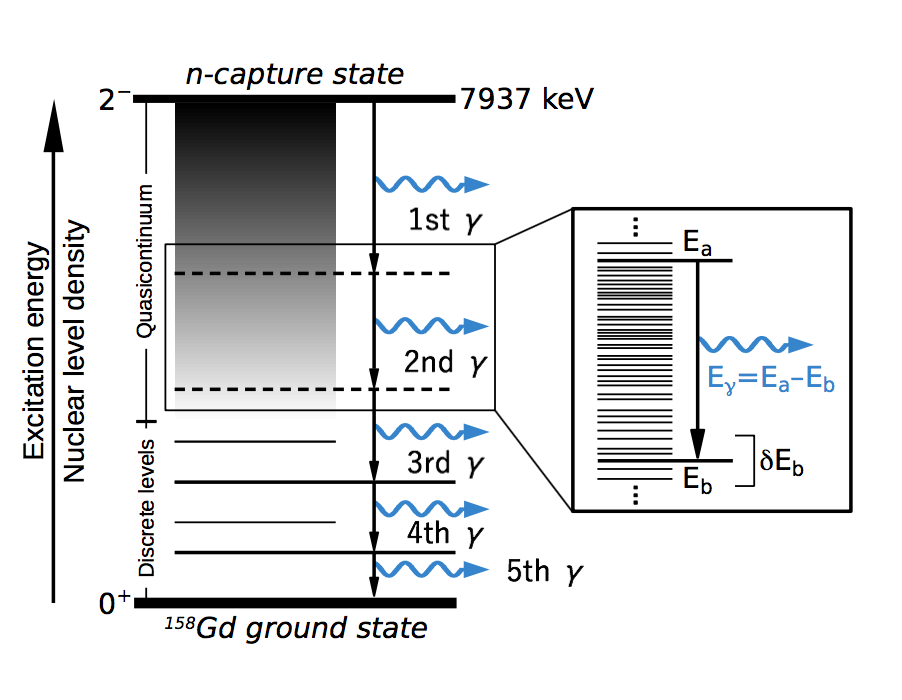
\includegraphics[width=0.6\linewidth]{figures/LZ/ContinuumEmission2.png}
    \caption{Illustration of the multi-step $\gamma$-ray emission of an excited $^{158}\text{Gd}^*$ following the thermal $^{157}\text{Gd}(n,\gamma)$ reaction. The de-excitation to the ground state can occur via many intermediate levels. Adapted from Ref.\cite{Hagiwara:2018kmr}.}
    \label{fig:Gd158Deexcite}
\end{figure}

In addition to neutron capture of Gd, hydrogen also produces a neutron capture signal. Hydrogen has thermal neutron capture cross section of 0.33~b which appears meagre in comparison with Gd, however due to the abundance of hydrogen in the LS, acrylic, and water, a significant number of neutron captures are observed. Following the capture of a thermal neutron, the excited deuterium atom decays to its ground state and emits a single 2.2~MeV $\gamma$-ray \cite{LZTDR}. The prominent peak resulting from the hydrogen capture can be in the OD energy spectrum, \autoref{fig:ODEnergySpec}.

\begin{figure}
    \centering
    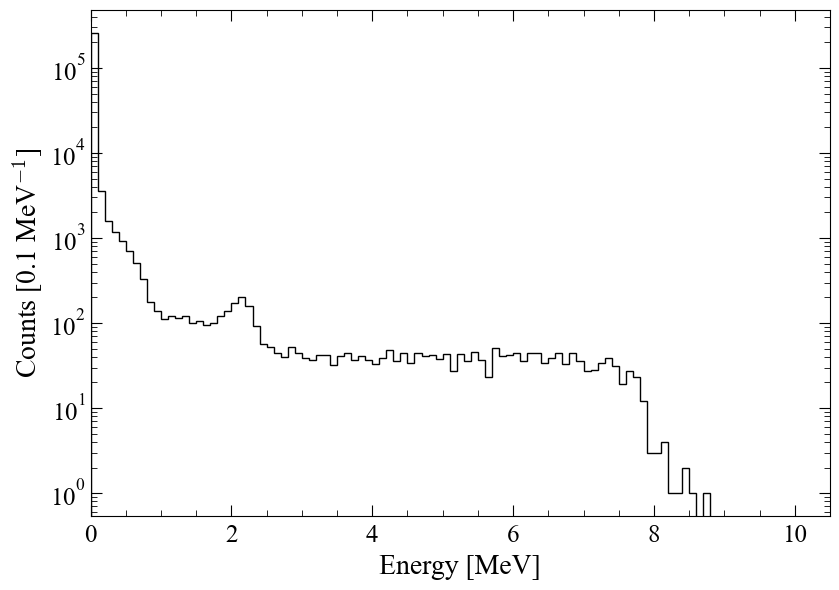
\includegraphics[width=0.7\linewidth]{figures/LZ/ODEnergySpec.png}
    \caption{AmLi energy spectrum measured with LZ Outer Detector with coincident single scatter signals in the TPC, here simple data quality cuts have been applied. The distinctive hydrogen capture peak can be seen at 2.2~MeV, whilst the continuous $\gamma$-ray spectrum from the Gd Capture has the expected end point at $\mathtt{\sim}$8~MeV.}
    \label{fig:ODEnergySpec}
\end{figure}

By doping LS with Gd, the efficiency for detecting at least one of the capture gammas is very high compared to having stand alone LS. Another advantage of Gd-doping is reduction in the time delay for neutron capture from $220\mu s$ to $28\mu s$ intern reducing the length of the window needed for vetoing by a factor of 7 \cite{LZTDR}. Detailed simulations by the LZ Collaboration initially expected to use a veto window of $125\mu s$, however it was found that neutrons also captured in the acrylic up to 10\% of the time \cite{LZTDR}. Further studies by the author also found that neutrons captured in the water which had partially saturated foam displacer between the acrylic tanks and OCV. This effect further extended the required veto window to $600\mu s$. This study is discussed further in \autoref{chap:VetoEfficiency}.

\subsection{PMT system}
Interactions in the GdLS and water are monitored by 120 Hamamatsu 8-inch R5912 photo-multiplier tubes (PMTs) arranged as shown in \autoref{fig:ODPMT_Array}. 
This model of PMT has been used successfully prior to their use in LZ at Daya Bay whose detector design is echoed in the LZ OD design \cite{Cao:2016vwh}. The R5912 PMTs were chosen because of the following reasons:
\begin{enumerate} 
    \item The spectral response ranges from 300~nm to 650~nm, with a peak wavelength at 420~nm. This encompasses the range of the scintillation light from the LAB mix between 390~nm to 440~nm \cite{Haselschwardt:2018vmp}. The comparison can be made comparing the plots in \autoref{fig:ODPMTSpecRes}.
    \item The quantum efficiency covers the relevant range, with an average expected value of $\sim25\%$ at 430~nm, as shown in \autoref{fig:ODPMTQE}.
    \item The radioactivity levels of the PMTs and support structure is a fairly weak constraint due to the 84~cm of water separating them from any active volume. In the scintillator itself, the simulated event rate from the PMT radioactivity is $<4~\text{Hz}$ \cite{LZTDR}. 
\end{enumerate}
\begin{figure}[ht!]
    \centering
    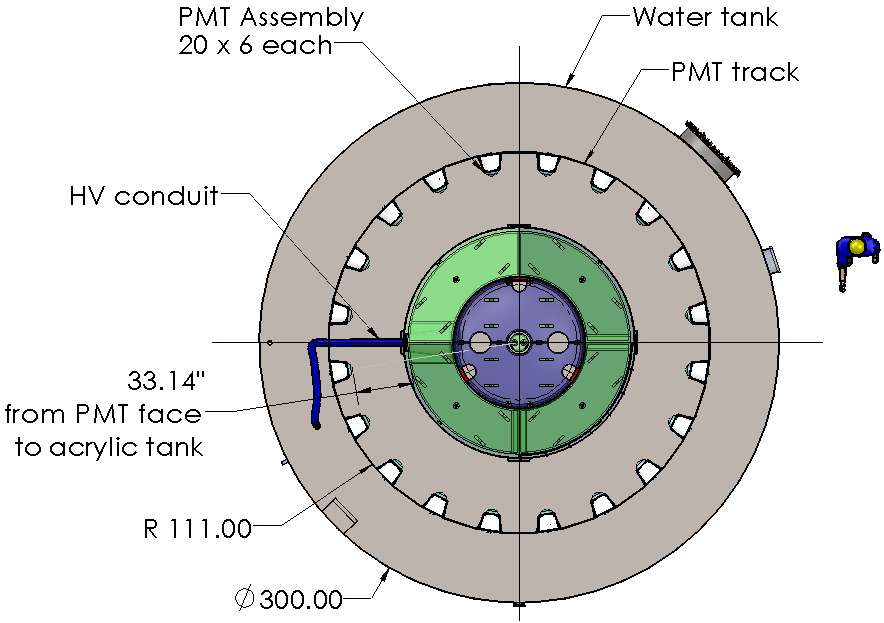
\includegraphics[width=0.6\linewidth]{figures/LZ/OD_PMT_support.jpg}
    \caption{Plan view of the OD PMT support system. The 20 PMT ladders are mounted to a circular track attached to the walls of the water tank \cite{LZTDR}.}
    \label{fig:ODPMT_Array}
\end{figure}
\begin{figure}
     \centering
     \begin{subfigure}{0.47\textwidth}
         \centering
         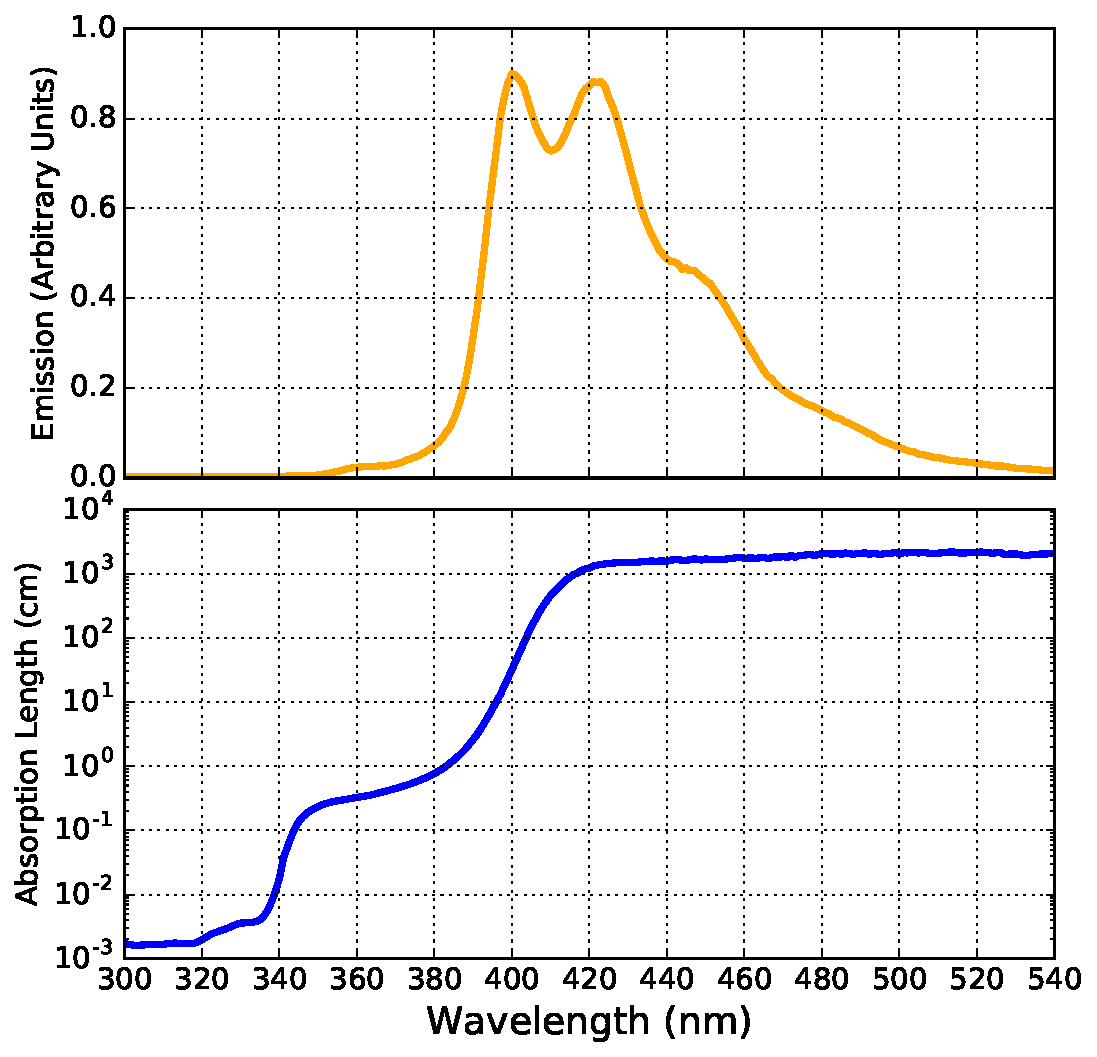
\includegraphics[width=\textwidth]{figures/LZ/GdLS_SpectralResponse.pdf}
         \caption{Wavelength dependence of two optical properties of the GdLS. \textbf{Top:} Emission spectrum of scintillation light. \textbf{Bottom:} The  absorption length of GdLS \cite{Haselschwardt:2018vmp}.}
         \label{fig:GdLSSpecRes}
     \end{subfigure}
     \hfill
     \begin{subfigure}{0.47\textwidth}
         \centering
         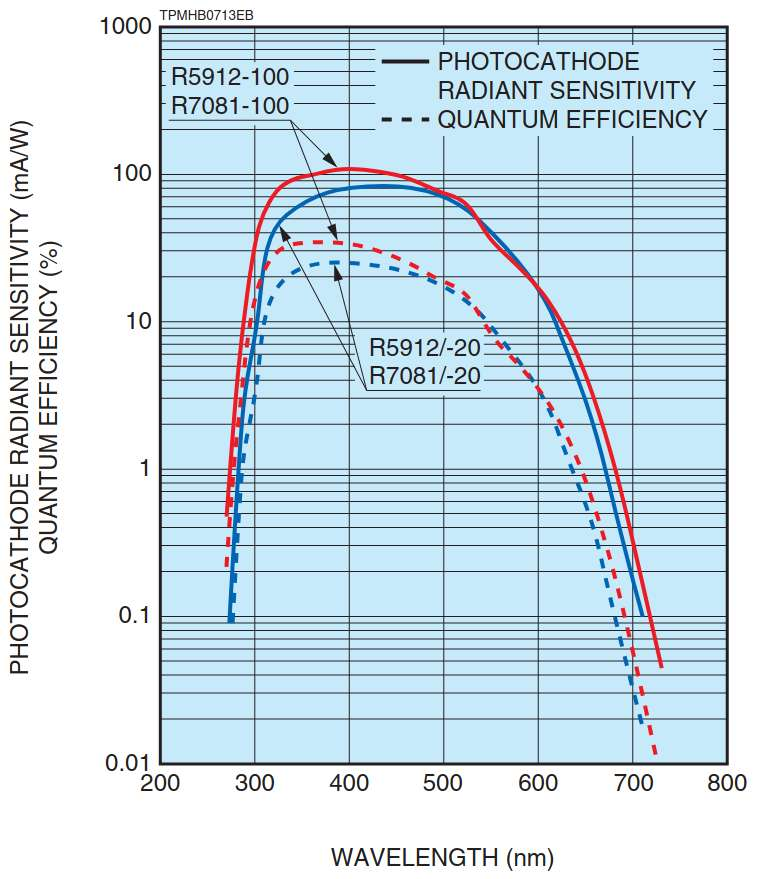
\includegraphics[width=\textwidth]{figures/LZ/ODPMT_QEvsWL.png}
         \caption{Wave length dependence of the quantum efficiency of the Hamamatsu 8-inch R5912 photo-multiplier tube. Adapted from Ref.\cite{HamamatsuR5912}}
         \label{fig:ODPMTQE}
     \end{subfigure}
     \caption{A comparison of the wavelength dependence of key optical parameters for both the GdLS and PMTs.}
     \label{fig:ODPMTSpecRes}
\end{figure}
Prior to the installation of the PMTs at SURF, rigorous testing to fully characterise the response of tubes was carried out by groups from Brandeis University and the IBS Center for Underground Physics. Further details of the quality assurance testing is documented in Ref.\cite{lkorley:thesis}.

\subsection{Outer Detector Optical Calibration System}
LZ uses an optical calibration system to monitor: the PMT gain/single photoelectron (SPhE) size; afterpulsing rates; and the optical properties of the acrylic and scintillator. Light produced by the LED-driven system is injected into the OD at 35 different locations. Thirty injection points are evenly distributed throughout the PMT array  (10 azimuthal positions at 3 heights as shown in \autoref{fig:OCSPositions}). Four of the injection points are each positioned in centre of the side acrylic tanks facing upwards to monitor the optical properties of the GdLS. One final injection points is positioned in the outer rim of a side acrylic tank also facing upwards and is used to monitoring the optical properties of the acrylic.
\begin{figure}
    \centering
    \includegraphics[width=\linewidth]{figures/LZ/OD_PMT_CAD_picture_v4.png}
    \caption{\textbf{Left:} A cross-section of a CAD drawing of the OD. The three  heights of the 10 azimuthal positions of the optical fibre injection points are labelled 1-3. Two injection positions under the side acrylic tanks which point upwards are labelled 4 and 5. \textbf{Right:} A photograph of the OD PMT array showing the point of an injection point relatively to the surrounding PMTs.}
    \label{fig:OCSPositions}
\end{figure}
Duplex fibres are used to inject light pulses produced by LEDs to the different locations. For the thirty injection points situated within the PMT, 435~nm LEDs are used to match the peak wavelength and quantum efficiency of OD PMTs. Only one core in the fibre is used, the additional core is a backup in the event of any damage to the first core. 435~nm and 450~nm were doing for the injection points facing into the LS to monitor optical degradation of the scintillator. Below 420~nm the absorption length of GdLS decreases significantly as shown in \autoref{fig:GdLSSpecRes}, if the scintillator degrades this region shifts to higher wavelengths.


\section{Calibration Sources}

\section{Data Acquisition System}

\section{Simulation Techniques}

\section{Assembly and Operation of the LZ Detector}